%\documentclass{emulateapj}
\documentclass[12pt,preprint]{aastex}
\usepackage{amssymb,amsmath}

\usepackage{verbatim}
\usepackage{color}
\slugcomment{Last revision \today.}

% A comment block

%\newcommand{\comment}[1]{}

% For color
\newcommand{\mpname}[1]{#1_color.eps}
\newcommand{\clraitoff}{red}
\newcommand{\lumblack}{(black)}
\newcommand{\lumblue}{(blue)}
\newcommand{\lumred}{(red)}
\newcommand{\vdisred}{(red-dashed curve)}
\newcommand{\vdisblue}{(blue-solid curve)}

% For bw
%\newcommand{\mpname}[1]{#1.eps}
%\newcommand{\clraitoff}{}
%\newcommand{\lumblack}{}
%\newcommand{\lumblue}{}
%\newcommand{\lumred}{}
%\newcommand{\vdisred}{(dashed curve)}
%\newcommand{\vdisblue}{(solid curve)}

\newcommand{\umag}{$u$}
\newcommand{\gmag}{$g$}
\newcommand{\rmag}{$r$}
\newcommand{\imag}{$i$}
\newcommand{\zmag}{$z$}
\newcommand{\gmr}{$g-r$}



\newcommand{\gammat}{$\gamma_T$}
\newcommand{\gammacross}{$\gamma_\times$}
\newcommand{\deltasig}{$\Delta \Sigma$}
\newcommand{\deltaplus}{$\Delta \Sigma_+$}
\newcommand{\deltacross}{$\Delta \Sigma_\times$}
\newcommand{\deltarho}{$\Delta \rho$}
\newcommand{\movr}{$M(<r)$}
\newcommand{\sigmacrit}{$\Sigma_{crit}$}

\newcommand{\photoz}{photo-z}
\newcommand{\photozs}{photo-zs}

\newcommand{\tlum}{$L^{tot}$}
\newcommand{\tngal}{$N_{gal}^{tot}$}

\newcommand{\lstarlim}{$0.4 L_*$}
\newcommand{\lvir}{$L_{200}$}
\newcommand{\nvir}{$N_{200}$}
\newcommand{\rvir}{$r_{200}^{gals}$}

\newcommand{\ngal}{$N_{gal}$}
\newcommand{\maxbcg}{maxBCG}
\newcommand{\numNgalBins}{12}
\newcommand{\numLumBins}{16}

\newcommand{\tngalAperture}{2$h^{-1}$ Mpc}

\newcommand{\photo}{\texttt{PHOTO}}
\newcommand{\astrop}{\texttt{ASTRO}}
\newcommand{\mt}{\texttt{MT}}
\newcommand{\spectro}{\texttt{SPECTRO}}
\newcommand{\spectroone}{\texttt{SPECTRO1d}}
\newcommand{\spectrotwo}{\texttt{SPECTRO2d}}
\newcommand{\target}{\texttt{TARGET}}

\newcommand{\lenszmax}{0.3}
\newcommand{\lenszmin}{0.05}

\newcommand{\photoversion}{\texttt{v5\_4}}

%\def\eone{e$_1$}
%\def\etwo{e$_2$}
\newcommand{\etan}{e$_+$}
\newcommand{\erad}{e$_\times$}
\newcommand{\eclass}{\texttt{ECLASS}}
\newcommand{\eclasscut}{-0.06}
\newcommand{\gmrcut}{0.7}

\newcommand{\hrs}{$^{\mathrm h}$}
\newcommand{\minutes}{$^{\mathrm m}$}

\newcommand{\ugriz}{$u, g, r, i, z$}
\newcommand{\polarization}{polarization}

\newcommand{\wgm}{$w_{gm}$}
\newcommand{\wgg}{$w_{gg}^p$}
\newcommand{\wmm}{$w_{mm}$}
\newcommand{\xigg}{$\xi_{gg}$}
\newcommand{\ximm}{$\xi_{mm}$}
\newcommand{\xigm}{$\xi_{gm}$}

\newcommand{\numspec}{127,001}
\newcommand{\numspecvlim}{10,277}
\newcommand{\numrand}{1,270,010}
\newcommand{\numspectot}{278,192}
\newcommand{\numvdis}{49,024}
%\newcommand{\numsource}{10,259,949}
% hirata: 
\newcommand{\nummask}{1,815,043}
\newcommand{\numTenMpc}{132,473}
\newcommand{\numThirtyMpc}{101,221}
\newcommand{\numsource}{27,912,891}

\newcommand{\numpairsTenMpc}{2,670,898,177}
\newcommand{\altnumpairsTenMpc}{2.7 billion}
\newcommand{\numpairsThirtyMpc}{14,818,082,122}
\newcommand{\altnumpairsThirtyMpc}{14.8 billion}



\newcommand{\xirmax}{$\xi_{gm}(R_{max})$}


\newcommand{\Lya}{Ly$\alpha$}
\newcommand{\Lyaf}{Ly$\alpha$~Forest}
\newcommand{\core}{\texttt{CORE}}
\newcommand{\bonus}{\texttt{BONUS}}
\newcommand{\primary}{\texttt{SURVEY\_PRIMARY}}
\newcommand{\known}{\texttt{KNOWN}}
\newcommand{\first}{\texttt{FIRST}}
\newcommand{\loz}{\texttt{LOZ}}
\newcommand{\cmass}{\texttt{CMASS}}

\shortauthors{Sheldon et al.}
\shorttitle{BOSS Target Selection}

\begin{document}

\title{Target Selection for the Baryon Oscillation Spectroscopic Survey}



\author{
Erin S. Sheldon,\altaffilmark{1}
Adam Myers,\altaffilmark{2}
Jo Bovy,\altaffilmark{3}
David W. Hogg,\altaffilmark{3}
Christophe Yeche,\altaffilmark{4}
and many others to be added
}

\altaffiltext{1}{Brookhaven National Laboratory, Bldg 510, Upton, New York 11973}
\altaffiltext{2}{Department of Astronomy, University of Illinois at Urbana-Champaign, 1002 W. Green St., Urbana, IL 61801-3074}
\altaffiltext{3}{Center for Cosmology and Particle Physics, Department of Physics, New York University, 4 Washington Place, New York, NY 10003.}
\altaffiltext{4}{CEA, Centre de Saclay, IRFU, F-91191 Gif-sur-Yvette, France}

\clearpage
\tableofcontents

\section{Introduction}


\section{SDSS Imaging Catalogs} \label{sec:sdssdata}

The input catalogs are derived from the imaging released as SDSS III Data
Release Eight \citep[SDSS DR8;][]{dr8}.   DR8 includes 2500 deg$^2$ of
additional imaging over data release seven, specifically acquired to aid in
spectroscopic target selection for \boss.

The creation of the imaging catalogs is mostly well described elsewhere,
including the derivation of photometric \citep{Nikhil08,Smith02,Tucker06}
and astrometric \citep{Pier03} calibrations, and calculation of basic
quantities such as fluxes and shapes \citep{LuptonADASS01}.  \citet{dr8}
also describe some new features in the DR8 dataset.

In the following sub-sections we will add some additional details about the
DR8 imaging dataset.

\subsection{Ubercal}

The catalogs are placed on the same relative photometric system using the
``ubercal'' technique described in \citet{Nikhil08}.  The relative calibration
is precise at the $\sim$1\% level.

There were small portions of the data used for target selection that were not
photometric.  We targeted these regions anyway because the tiling algorithm
(XXX) cannot find an efficient solution in the presence of holes that are
comparable to the tile size.  This effectively means that the target selection
is not uniform over the entire survey, even in the cases where a uniform
algorithm was applied.  

We have developed a \mangle\ \citep{SwansonMangle08} mask to mark these and
other regions of sky we wish to ignore in science analyses that depend on a
good understanding of the underlying selection function, such as angular
correlations.  It is recommended that users make use of these masks when
performing statistical studies using the \boss\ spectroscopic samples.  See \S
\ref{sec:masks} for details of these masks and how to obtain them. 

\subsection{AB Zero Points}

{\color{red} Do we have any knowledge of this?  David suggests we know it only
vicariously through matching to dr7 and demanding consistency.}

Daniel 1152

\begin{verbatim}
u(AB) = u(SDSS) - 0.036 - 0.009
g(AB) = g(SDSS) + 0.012 - 0.004
r(AB) = r(SDSS) + 0.01 by assumption
i(AB) = i(SDSS) + 0.028 + 0.002
z(AB) = z(SDSS) + 0.04ish + 0.004
\end{verbatim}

Marriner 1339


\begin{verbatim}
u=-0.037
g=+0.024
r=+0.005
i=+0.018
z=+0.016
\end{verbatim}

\subsection{Cataloged Quantities}

In this section we describe the quantities from the imaging catalogs used in
target selection.    These are all described in the above references, but we
will give a few more details here.

\subsubsection{Flux Measurements}

We use a few different fluxes in our selection. For point sources we always use
the flux derived by fitting a model of the local PSF interpolated to the
location of the object \citep{LuptonADASS01,Sheldon04}, known as \psfmag.  


For galaxies we use three different magnitudes, one optimized for colors called
\modelmag\footnote{\DRatemags}, one designed to be an approximate total
magnitudes in each band, called \cmodelmag, and one designed to mimic
the 2 arcsec aperture of the spectroscopic fibers called \fibertwomag.  

We fit each object to elliptical exponential disk and elliptical \devauc\
models, convolved with a double Gaussian approximate to the PSF model
interpolated to the location of the object.  The best fit model in the
\rmag-band is then used to measure fluxes in the other bands, convolving with
the filter-dependent PSF as appropriate.  Because the effective aperture is the
same for each band, \modelmag\ is appropriate for measuring colors.  

Note, as part of the \devauc\ fitting we measure the scale radius $r_{deV}$
which is also used in galaxy target selection.

For approximate total magnitudes, we use ``composite model magnitudes'', aka
\cmodelmag.  In \photo\ we do an additional joint fit to a non-negative linear
combination of the best-fitting exponential and \devauc\ models.  The parameter
\texttt{frac\_deV} ($f_{deV}$) is then used to construct \cmodelmag\ from the
individual fits.
\begin{equation}
\textrm{Flux}_{cmodel} \equiv (1-f_{dev})\times \textrm{Flux}_{exp} + f_{dev} \times \textrm{Flux}_{dev},
\end{equation}

The \fibertwomag\ is the flux in a 2 arcecond aparture, convolved with a 2
arcsecond PSF model in order to simulate the expected seeing during
spectroscopic observations.  The \fibertwomag\ is used as a faint end cut for
galaxy targets.

\subsubsection{Image Processing Flags}

flags,objc\_flags,objc\_flags2 Lets just call these OBJECT and be explicit when
it is applied to all bands as objc

calib\_status not used...

\subsubsection{Other Quantities}
\begin{verbatim}
ra,dec
rowv,colv
\end{verbatim}

\subsection{Unique Object Selection}

The selection of unique objects from the imaging data, which we call the
\texttt{resolve}, is described in detail in \citet{dr8} as well as the SDSS3
website\footnote{\DRateresolve}.  In the following sections, we refer to the
use of the \texttt{SURVEY\_PRIMARY} bit in the \texttt{RESOLVE\_STATUS}, which
marks these unique objects.


\section{Initial Star-Galaxy Separation} \label{sec:sgsep}

Inital star galaxy separation is performed in the photometric pipeline \photo.
The algorithm uses only morphological information.  We first define
the concentration $c$ as the difference between the 
\psfmag\ and \modelmag:
\begin{equation}
c \equiv \textrm{psfmag} - \textrm{modelmag}~.
\end{equation}
The fluxes are summed for all bands.  Because the exponential and
\devauc\ models are convolved with the local PSF, the model scale radius
approaches a delta function for stars, and $c$ approaches zero.  The measured
concentration for galaxies should be greater than zero.  We define a simple cut
$c > 0.145$ for galaxies.  For the galaxy \loz\ sample we add an additional
cut in the \rmag-only concentration at 0.3, to be consistent with 
the Luminous Red Galaxy sample from SDSS I (cite XXX).

We implemented an alternative star galaxy separation scheme for the \cmass\
galaxy target selection using only \imag-band, which should be more
well-measured than bluer bands for our galaxy targets. We did not see
significant improvement.

Note the star sample is used as a starting point for quasar target selection.
This simple concentration cut is not adequate at the faint magnitudes
(\gmag$\sim 22$) used for quasar selection\footnote{see, e.g., \DRsevsg}.
However, the color based selection reduces the contamination by galaxies and in
fact stars are by far the largest contaminant in the quasar target sample
\citep{RossQTS}.


\section{Galaxy and Star Pre-selection}

\subsection{Basic Quality Cuts}

We use as the starting point for our selection the \calibObj\ or ``datasweep''
files.   These files contain only objects that meet certain basic criteria.
First, basic star-galaxy separation is performed.  For objects marked as stars,
we only retain those objects with extinction-corrected \psfmag\ less than
[22.5, 22.5, 22.5, 22, 21.5] in the \allmag\ bands, respectively.  For
galaxies, we retain objects with extinction-corrected \modelmag\ less than [21,
22, 22, 20.5, 20.1].

\subsection{Masks and Survey Boundaries} \label{sec:masks}

Describe use of mangle (cite XXX).

Describe corrected survey coordinates, the system used for defining masks.

Objects outside the \boss\ survey boundaries are not considered for
spectroscopic followup. Figure XXX shows the outline of this boundary
separately for the NGC and SGC.

\begin{figure}[t] \centering
 \centering 
 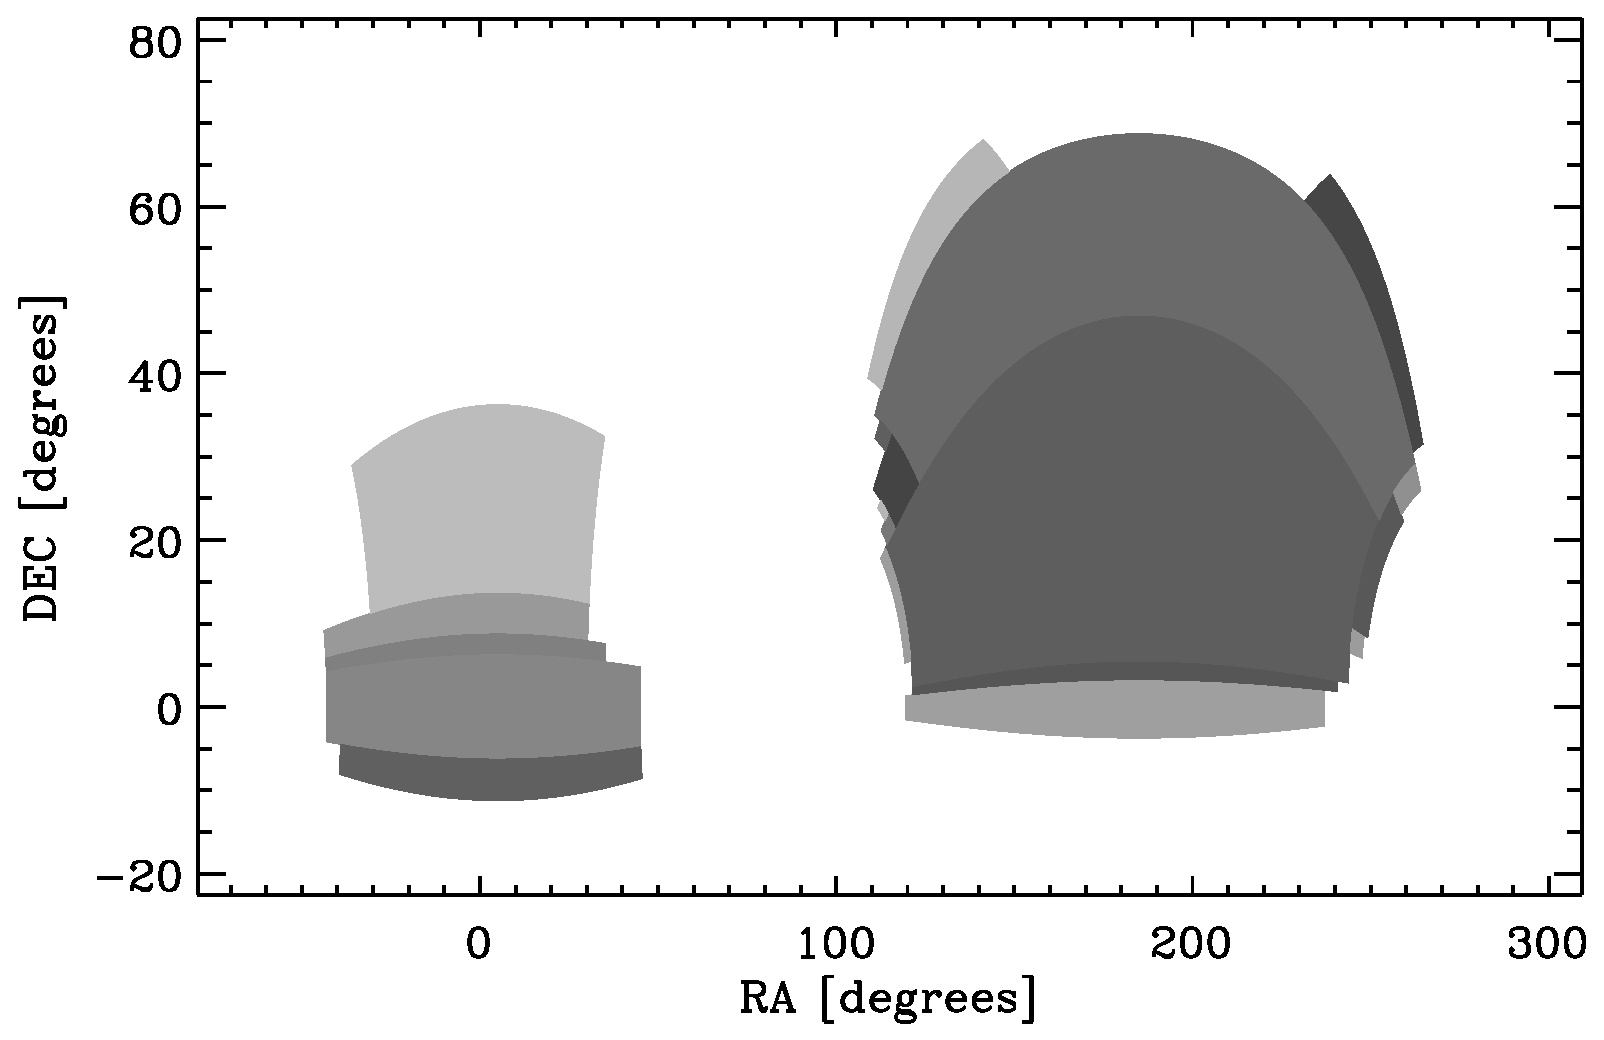
\includegraphics[scale=0.6]{fig/boss-poly-coverage.eps}

 \caption{BOSS angular window function for the south galactic cap on the left
 and the north galactic cap on the right.  The differently shaded regions
 represent contiguous rectangular regions in SDSS survey coordinates, used for
 construction of the window function.  Note points with RA $>$ 300\arcdeg\ have
 been wrapped below zero to avoid the 360\arcdeg\ crossing point.}
 \label{fig:footprint}

\end{figure}



In addition to this overall boundary cut, we masked regions where the certain
amplifiers on chips behind \umag\ filters were not functioning (XXX need more
info on this failure).  These regions are all in the NGC and are shown in XXX
in figure XXX.

\subsection{Datasweeps} \label{sec:sweeps}


\subsection{Coadds}


\section{Target Selection Framework}

\subsection{Structure of Software Pipeline} \label{sec:structure}

Describe how we actually do the processing.

\subsection{General Photometric Selection} \label{sec:genselect}

Objects that do not meet certain criteria are removed from consideration for
spectroscopic followup. The only exceptions to this are certain known quasar
objects, which are subjected to less restrictive criteria (see \S
\ref{sec:knownfirst}), and quasars selected from coadded data during
commissioning (XXX need Christophe's criteria).


The following are not considered for spectroscopic followup:

\begin{itemize}

    \item Objects not labeled as \primary.

    \item Objects outside the BOSS footprint.

    \item Objects labeled as \texttt{BRIGHT}.

    \item Objects labeled as \texttt{SATUR}.

    \item For quasars and standard stars, objects
        labeled as \texttt{INTERP\_CENTER}, 
        \texttt{PSF\_FLUX\_INTERP}

    \item For galaxies and quasars, objects labeled
        as \texttt{NOTCHECKED}, for standards labeled
        as \texttt{NOTCHECKED\_CENTER}.

    \item For galaxies and quasars, objects labeled as
        \texttt{PEAKCENTER}.

    \item For galaxies and standard stars, objects labeled
        as \texttt{NOPROFILE}.

    \item For galaxies and standard stars, objects labeled as 
        \texttt{DEBLEND\_TOO\_MANY\_PEAKS}.

    \item For quasars and standard stars, objects that have
        a cosmic ray in an associated pixel \texttt{CR}.
    
    \item For quasars and standards, objects labeled
        as \texttt{BLENDED}, for galaxies objects labeled
        as \texttt{BLENDED} but also \texttt{NODEBLEND}.


    \item For quasars, objects not labeled as \texttt{BINNED1} in some band, 
    for galaxies not labeled as \texttt{BINNED1}, \texttt{BINNED2}
    or \texttt{BINNED4} either the \rmag- or \imag-band.
   
\end{itemize}

\section{Standard Star Selection Framework} \label{sec:std}

In addition to those cuts listed in \ref{sec:sweeps} and \ref{sec:genselect},
the following are not considered for followup as standard stars:

\begin{itemize}

    \item Objects that have bad sky measurements \texttt{BADSKY}.
    \item Objects labeled to have \texttt{PEAKS\_TOO\_CLOSE}.
    \item Objects not labeled as \texttt{STATIONARY}.
    \item Known quasars.
   
\end{itemize}



\section{Galaxy Selection Framework} \label{sec:galframe}

\subsection{Galaxy Photometric Cuts}

In addition to those cuts listed in \ref{sec:sweeps} and \ref{sec:genselect},
the following are not considered for followup as galaxies:

\begin{itemize}



    \item Objects within a specified distance of a known Tycho star
    \citep{tycho2}.  The distance is magnitude dependent, and is given 
    by
    \begin{equation}
    r = (0.0802\times B_T^2 - 1.860\times B_T + 11.625)/60.0,
    \end{equation}
    where $B_T$ is the Tycho magnitude and $r$ is in degrees.

    \item Galaxies that already have known redshifts from the SDSS.

    \item The object is a known quasar or star.

\end{itemize}

\subsection{Galaxy Selection Algorithms}

Show formulas and some status, heat maps, etc.



\section{QSO Selection Framework} \label{sec:qsoframe}

In this section, we describe the overarching framework of the BOSS
quasar target selection algorithm. The algorithm is complex, motivated
by the primary goal of the BOSS QSO survey --- to measure the baryon
acoustic feature in the \Lyaf\ --- while additionally maintaining a more
generally useful sample for the community.

\subsection{QSO Selection Algorithms}

The primary science goal of the BOSS QSO survey is to detect and measure
the baryon acoustic feature in large-scale structure as traced by
the \Lyaf. A complex angular selection function is not in general a
hindrance to this measurement, as most of the information is in the
flux power spectrum along the lines of site rather than in angular
correlations.

In addition to the focus on \Lyaf, BOSS will assemble an unparalleled
collection of quasars at $2 < z < 4$, potentially making a range of new
statistical studies possible in the moderate-redshift universe.

To address both of these considerations, the BOSS quasar targeting
framework was effectively divided into two algorithms. The first
algorithm uses only objects marked as \primary\ in the single-epoch
data (see \S \ref{sec:sdssdata}), and uses a single tunable parameter
for target selection. The resulting sample is called the \core\ sample.
Because this sample is uniformly selected from homogeneous data, it is
useful for statistical quasar studies such as population and angular
clustering.

The second algorithm we leave free to incorporate multi-epoch data from 
the SDSS imaging, as well as any other data at hand, such as that
from external surveys that may improve the signal derived from
the \Lyaf.  The resulting sample is called \bonus.  This sample
may continue to change over time -- sufficiently to render 
descriptions of \bonus\ in this document obsolete.

Along with \core\ and \bonus, two other main algorithms are used in BOSS
quasar target selection. The first includes or excludes sources based on
whether they are known quasars or stars from other surveys. The second
includes objects based on whether they have a match to an object in the
FIRST radio survey. We refer to these algorithms as \known\ and \first\
respectively.  

The details of the above samples will be described in more detail in


\subsection{Common Photometric Cuts for QSOs}

As listed below, the \core\ and \bonus\ algorithms share a set of cuts on the
SDSS photometry. These cuts are applied in addition to those listed in \S
\ref{sec:genselect}. Exceptions are \known\ and \bonus\ from commissioning,
which will be described later.

In addition to those cuts listed in \ref{sec:sweeps} and \ref{sec:genselect},
the following are not considered for followup as QSOs:

\begin{itemize}

    \item Objects labeled as \texttt{BAD\_COUNTS\_ERROR}.
    \item Objects labeled as \texttt{DEBLEND\_NOPEAK}.
    \item Objects labeled as \texttt{EDGE}.
    \item Objects labeled as \texttt{DEBLENDED\_AS\_MOVING}.

\end{itemize}

\subsection{The QSO \known\ and \first\ Algorithms} \label{sec:knownfirst}

\subsection{The QSO \core\ Algorithm}

During Year~1 of the survey, the definition of \core\ was altered several times
to attempt to optimize return within the statistical sample of BOSS quasars.
Here, we show results for the final definition of \core, derived near the
beginning of Year~2, which uses the Extreme Deconvolution method of
\citet{BovyQSOPhotoz2011}.  The \core\ algorithm will not change further.

Show some heat maps, density histograms, etc.

\subsection{The QSO \bonus\ Algorithm}

Here we describe results for the QSO \bonus\ as it existed at the beginning
of Year~2.  The definition of \bonus\ will change throughout the survey.

Show some heat maps.


\section{Target Lists Used During Observations}

Describe comm, comm2, main* etc, and which chunks these were used for.  Don't
worry that the algorithms changed and are not reflected in the stats and plots
shown above.

\section{Success Rate}

Discuss the success rates for QSO \core\, \bonus\, \first\ and galaxies.
Need to use most relevant data for this.

\section{Discussion}


\begin{comment}
The quasar candidates are broken into two samples: the ``core'' and the
``bonus''. The core sample is intended to be a nearly uniform selection,
both spatially and temporally throughout the survey. This uniformity
will facilitate statistical studies of their spatial distribution and
population. The bonus sample is designed to maximize the value for LyA
studies; uniformity is not a priority.

As with the galaxies, during commissioning we experimented with
selection at higher target density in order to better explore the
parameter space. 
(XXX get text from Adam describing the history of core)
Currently the core sample is set by a subset of the likelihood
method (see \S \ref{sec:like}) tuned to \~ 20/sq degree.

For the bonus sample, we use multiple algorithms to select quasar
candidates. As detailed in the quasar target selection paper (cite XXX),
there is significant overlap between the algorithms, but each also
selects a unique set of real quasars. The methods are combined in order
to boost the total completeness using a neural network ``combinator'', 
as outlined in \S \ref{sec:comb}.

Below we will describe briefly the core likelihood algorith, as well as
each algorithm used for the bonus sample and the method for combining
them.


\subsection{Likelihood} \label{sec:like}

\subsection{Artificial Neural Network} \label{sec:nn}

We use an Artificial Neural Network (ANN) at two stages of the selection
process. During the second stage we use an ANN as a ``combinator''
to select the best of the best from the individual algorithms. We
will outline this method in \S \ref{sec:comb}. The first use of the
ANN, which we outline here, works directly on the fluxes as do the
other algorithms. The full details of this algorithm can be found in
\citet{yeche10}.

The ANN uses all fluxes and errors to produced a single likelihood that
the object is a quasar.
The basic building block of the ANN architecture
is a processing element called a neuron.
The ANN architecture used in this study is 
illustrated in Fig.~\ref{fig:ArchitectureNN}, where
each neuron is placed on one of four ``layers'', 
with $N_l$ neurons in layer $l,\,l=1,2,3,4$.
The output of each neuron on the first (input) layer is 
one of the $N_1$ variables defining an object,
e.g., magnitudes, colors, and uncertainties.
The inputs of neurons on subsequent layers ($l=2,3,4$) are the $N_{l-1}$ outputs of the
previous layer, i.e., the $x^{l-1}_j ,\,j=1,..,N_{l-1}$.
The inputs of any neuron are first linearly
combined according to ``weights'', $w^l_{ij}$ and ``offsets''
$\theta^l_j$ 

\begin{equation}
y^l_j=\sum_{i=1}^{N_l} w^l_{ij}\, x^{l-1}_i +  \theta^l_j\,\,
\hspace*{5mm}l\,\geq\,2 \;.
\end{equation}
The output of neuron $j$ on layer $l$ is then defined by the 
non-linear function
\begin{equation}
x^{l}_j 
=
%\left[ 
\frac{1}{1+ \exp\left(-y^l_j\right)}\,\,
\hspace*{5mm} 2\leq \,l\,\leq 3 \;.
%\right]^{-1}
%=\frac{1}{1+ e^{-y_l}}
\label{eq:activation}
\end{equation}
The fourth layer has only one neuron giving an output  $y_{NN}\equiv y^4_1$,
reflecting the likelihood
that the object defined by the $N_1$ input variables is a QSO.              

\begin{figure}[htb]
  \centering
 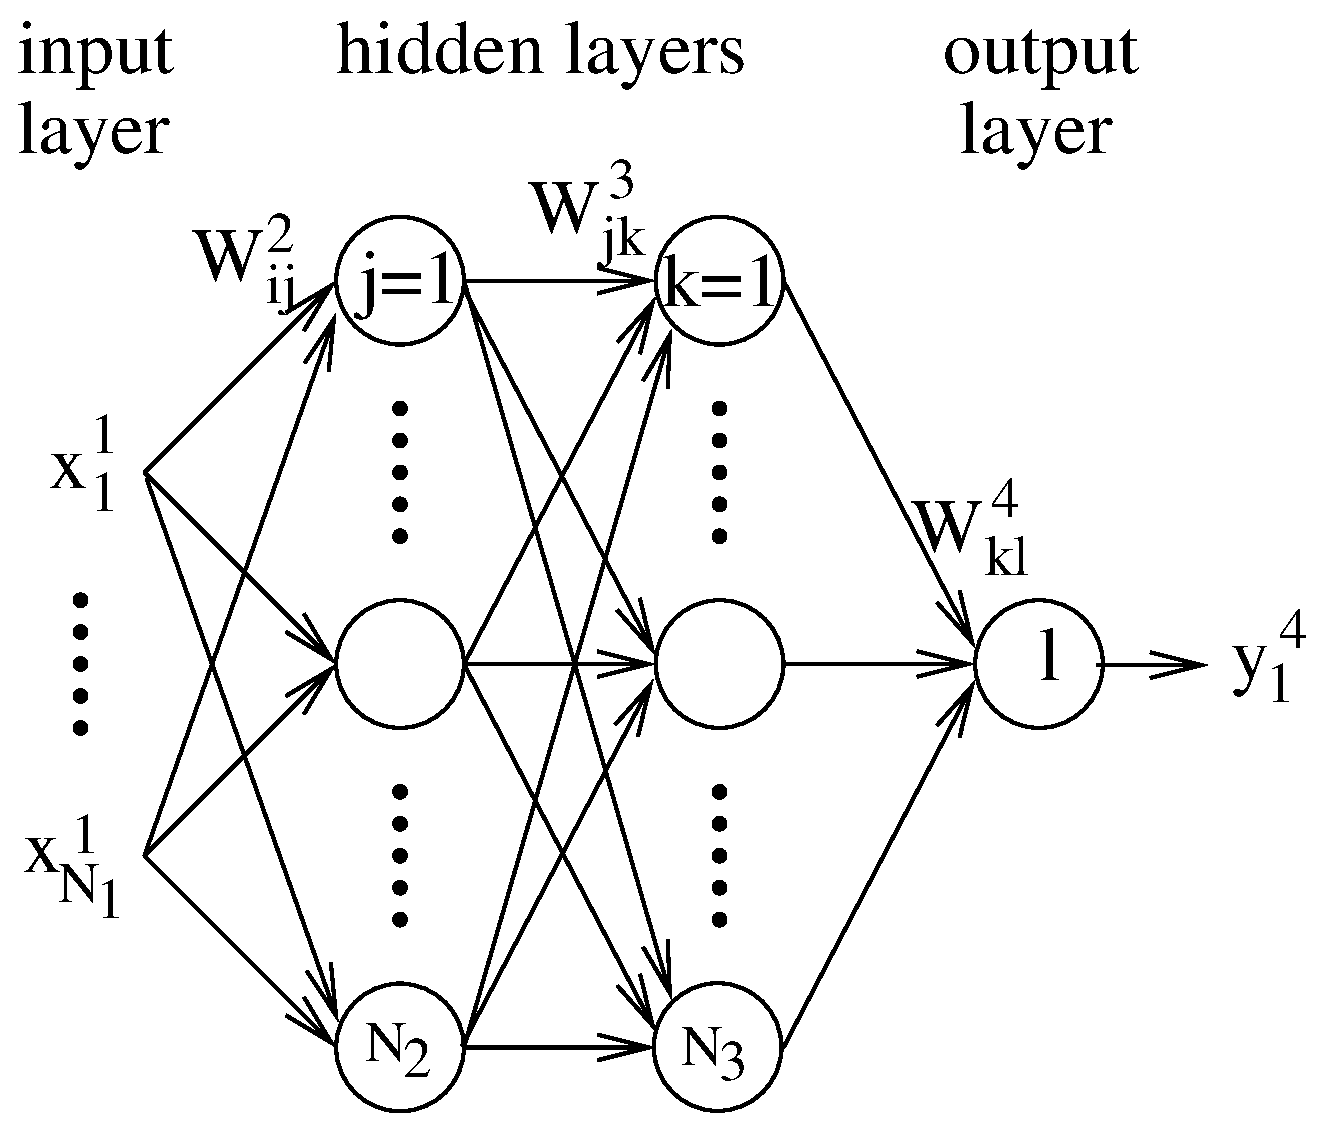
\includegraphics[width=7.cm]{fig/SchemaNN.eps}
     \caption{ Schematic representation of the artificial neural network used here with 
$N_1$  input variables, two hidden layers, and one output neuron.}
        \label{fig:ArchitectureNN}
  \end{figure}


 \begin{figure*}[htb]
  \centering
  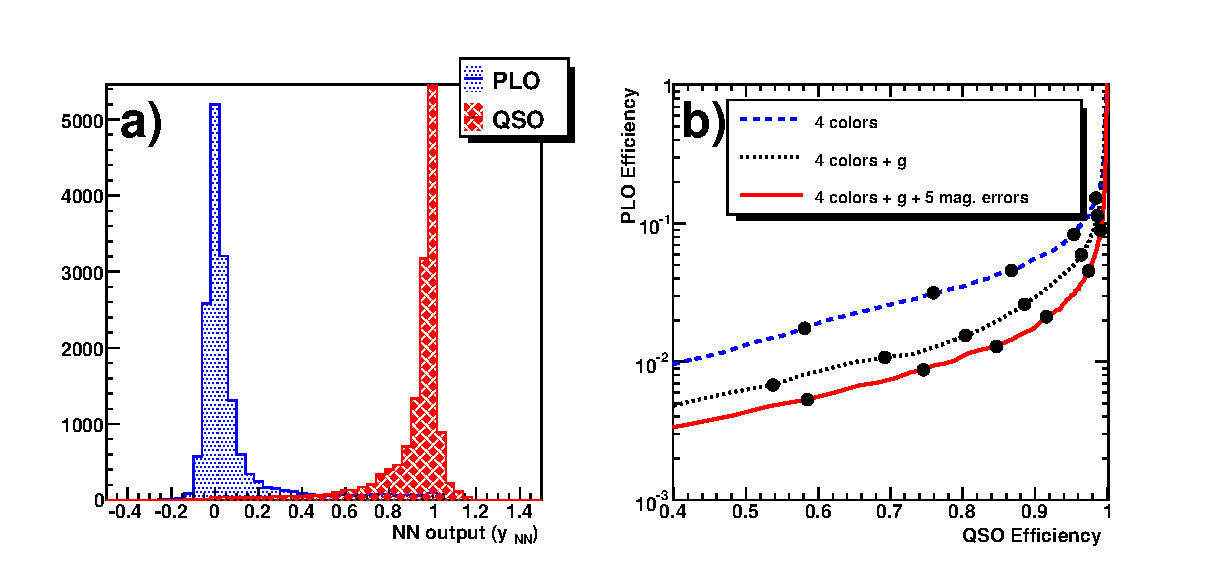
\includegraphics[width=\textwidth]{fig/NNOutputEffi.eps}
     \caption{{\bf a)} ANN output for  objects classified as PLO in the SDSS photometric catalog, 
i.e. background objects, (blue dotted histogram) and for objects 
spectroscopically classified as QSO (red slashed histogram) in the control samples,
using 10 variables: 4 colors, $g$ magnitude, and errors in the 
five ($u,g,r,i$ and $z$) magnitudes.
{\bf b)} PLO efficiency 
%(fraction of selected PLOs) 
as a function of the 
QSO efficiency 
%(fraction of QSOs in the output sample) 
for three ANN configurations. 
Blue dashed line: 4 colors ($u-g,g-r,r-i,i-z$). Black dotted line: 4 colors + $g$ magnitude. Red 
solid line: 4 colors + $g$ magnitude + errors in the five  ($u,g,r,i$ and $z$) 
magnitudes. The curves are obtained by varying the cut value, $y^{min}_{NN}$
for the two distributions of Fig.~\ref{fig:NNOutputEffi}-a. Efficiency is defined 
as the ratio of the number of objects with a ANN output greater than $y^{min}_{NN}$ to
the number of objects in the sample. The dots correspond, from left to right, 
%the PLO efficiency as a function of QSO efficiency,  for 
to $y^{min}_{NN}$ equal to, respectively, 0.2, 0.5, 0.8, 0.9, 0.95, and 0.98. }
        \label{fig:NNOutputEffi}
  \end{figure*}

Certain aspects of the ANN procedure, especially the number of layers and the 
number of nodes per layer, are somewhat arbitrary and are chosen by experience
and for simplicity.
On the other hand, the weights and offsets must be optimized so that
the ANN output, $y_{NN}$,  correctly reflects the probability
that an input object is a QSO.        
The ANN must therefore be ``trained''
with a set of objects that are known
to be either QSOs or not QSOs (background objects).
More precisely, the weights and offsets are determined by minimizing the ``error'' function
\begin{equation}
E= \frac{1}{2n}\sum_{p=1}^{n}(y_{NN}(p)-y(p))^2\,\, ,
\label{eq:error}
\end{equation}
where the sum is over $n$ objects, $p$, and where $y(p)$ is a discrete value
defined as  $y(p)=1$ (or $y(p)=0$) if the
object $p$ is a QSO (or is not a QSO). When the ANN is developed 
to estimate a photometric redshift, the targeted value $y(p)$ is a continuous value 
equal to the true spectrometric redshift, $z_{spectro}$. 

In this kind of classification analysis, the major risk is the
``over-training'' of the ANN. It occurs when the ANN has too many
parameters ($w_{ij}$ and $\theta_j$) determined by too few training
objects. Over-training leads to an apparent increase in the
classification efficiency because the ANN learns by heart the objects in
the training sample. To prevent this behavior, the QSO and background
samples are divided into two independent subsamples called ``training''
and ``control'' samples. The determination of the ANN parameters
($w_{ij}$ and $\theta_j$) is obtained by minimizing the error $E$,
computed over the QSO and background training samples. The minimization
is halted as soon as the error in the control samples stops decreasing
even if the error continues to decrease in the training samples.
We followed this procedure for both the target selection and the
determination of the photometric redshift.


The background sample used in the training of the ANN was drawn from
the SDSS Point Like Object (PLO) sample. We used objects with Galactic
latitude $b$ around $45^\circ$ to average the effect of Galactic
extinction. In the future, we may consider the possibility of having a
different ANN for each stripe of constant Galactic latitude. The final
sample contains ~30000 PLOs.

For the QSO training sample, we used a list of 122818
spectroscopically-confirmed quasars obtained from the 2QZ quasar
catalog \citep{croom04}, the SDSS-2dF LRG and QSO Survey (2SLAQ)
\citep{croom09}, and the SDSS-DR7 spectroscopic database \citep{dr7}.
These quasars have redshifts in the range $ 0.05 \leq z \leq 5.0
$ and $g$ magnitudes in the range $18 \leq g \leq 22$ (Galactic
extinction-corrected). Since quasars will be observed over a limited
blue wavelength range (down to about 3700~\AA), we targeted only quasars
with $z>2.2$. Therefore, the sample of known quasars includes 33918 QSOs
with $z\geq 1.8$.

The result of the ANN training procedure is shown in
Fig.~\ref{fig:NNOutputEffi}-a. The histograms of $y_{NN}$ for the
control QSO and background samples are overplotted. Most objects
have either $y_{NN}\sim 1$ (corresponding to QSOs) or $y_{NN}\sim 0$
(corresponding to background objects). QSO target selection is achieved
by defining a threshold value $y_{NN}^{min}$ to be chosen between
$y_{NN}= 1$ and $y_{NN}\sim 0$. The optimal value of the threshold is
obtained by balancing the number of accepted QSOs against the number of
accepted background objects. A plot of the QSO efficiency versus the
background efficiency is shown in Fig.~\ref{fig:NNOutputEffi}-b.



\subsection{Extreme Deconvolution} \label{sec:exd}


The extreme-deconvolution quasar target selection technique
\citep[XDQSO;][]{bovy11} uses the extreme deconvolution method 
\citep[XD;][]{Bovy09} to build a model of the distribution of relative
fluxes---relative to $i$---of stars and quasars in different redshift
ranges based on training samples of known stars and quasars. XDQSO
deconvolves the relative-flux distribution by modeling it as a mixture
of 20 Gaussian components and fitting this model to the training data,
taking the heteroscedastic nature of the SDSS flux uncertainties
fully into account. The XD model for the relative-flux distribution
is fit in narrow bins in $i$ band magnitude and combined with an
apparent-magnitude dependent prior based on star counts in stripe-82 and
the \citet{Hopkins07} quasar luminosity function.

The probability for an object to be a mid-redshift quasar ($2.2 \leq
z \leq 3.5$) is obtained as the ratio between the number density of
mid-redshift quasars and that of stars plus all quasars at the object's
fluxes. The probability for a single class is
%\begin{equation}
\begin{multline}
P(\mathrm{QSO}_{\mathrm{midz}} | \{\mathrm{F}_k\}) \propto \\
 P(\{\mathrm{F}_k/\mathrm{F}_i\} | \mathrm{QSO}_{\mathrm{midz}})\,
 P(\mathrm{F}_i | \mathrm{QSO}_{\mathrm{midz}})\,P(\mathrm{QSO}_{\mathrm{midz}})\,,
\end{multline}
%%\end{equation}
where $k$ indexes the fluxes and $\mathrm{F}_i$
is the SDSS \imag-band flux. The first factor on the right is
given by the XD model for the relative-flux distribution and the
second and third factors are obtained from the quasar luminosity
function. The underlying relative-flux distribution is convolved with
the object's flux uncertainties before evaluation. The expressions
for stars and high/low redshift quasars are similar. Probabilities
are normalized assuming that these classes exhaust the possibilities
($P(\mathrm{QSO}_{\mathrm{midz}}) + P( \mathrm{QSO}_{hiloz}) + 
P(\mathrm{star}) = 1$). Objects are ranked on their
mid-redshift quasar probability for targeting.

Since XDQSO target selection properly takes the flux uncertainties
into account both in the training and the evaluation stage, it
can be trained and evaluated on low signal-to-noise data. We have
trained XD models both on SDSS $ugriz$ fluxes alone and
SDSS+GALEX FUV and NUV \citep{bovy11}.

\subsection{$\chi^2$ Method} \label{sec:chi2}

\subsection{Kernel Density Estimate} \label{sec:kde}

\subsection{The ``Combinator''} \label{sec:comb}

\end{comment}

\acknowledgements E.S. is supported by grant DE-AC02-98CH10886.
J.B. and D.W.H. were partially supported by NASA
(grant NNX08AJ48G) and the NSF (grant AST-0908357). D.W.H. is a
research fellow of the Alexander von Humboldt Foundation of Germany.



\bibliographystyle{apj}
% Bib database
\bibliography{apj-jour,astroref}


\begin{comment}
\begin{thebibliography}{}
\bibitem[Bovy, Hogg, \& Roweis(2009)]{Bovy09a}
{Bovy}, J., {Hogg}, D.~W., \& {Roweis}, S.~T. 2009, {arXiv:0905.2979v1
[stat.ME]}
\bibitem[Hopkins, Richards, \& Hernquist(2007)]{Hopkins07a}
  Hopkins,~P.~F., Richards,~G.~T., \& Hernquist, L., 2007,
  \apj, 654, 731
\end{thebibliography}
\end{comment}

\end{document}
